\باب{تکمل کا استعمال}

\موٹا{مجموعی جائزہ}\quad
ہم بہت سی معلومات کو تکمل کی مدد سے حاصل کر سکتے ہیں: منحنیات کے بیچ رقبہ، ٹھوس اجسام کے حجم اور سطحی رقبے، منحنیات کی لمبائیاں، زیر زمین پانی کی نکاسی کے لئے درکار کام، سیلاب دروازوں پر اثر انداز قوتیں، ٹھوس اجسام کے نقطہ توازن کے محدد۔ ان تمام کو ہم بند وقفوں پر استمراری تفاعل کے ریمان مجموعوں کے حد یعنی تکمل سے ظاہر کر کے ان حدوں  کو  احصاء سے حل کرتے ہیں۔

عملی استعمال میں ان قطعی تکمل کو ایک مخصوص طرز سے لکھا جاتا ہے جس کو سیکھ کر بوقت ضرورت  نئے تکمل لکھے جا سکتے ہیں۔ مخصوص عملی استعمال پر پہلے غور کیا جائے گا۔ اس کے بعد تکمل لکھنے کی طرز پر اور نئے تکمل لکھنے پر غور کیا جائے گا۔

\حصہ{منحنیات کے بیچ رقبہ}
محددی مستوی میں خطے کی سرحدوں کو ظاہر کرنے والے تفاعل کے تکمل سے خطہ کے رقبہ کا حصول اس حصے میں دکھایا جائے گا۔

\جزوحصہء{بنیادی کلیہ بطور ریمان مجموعوں کا حد} 
فرض کریں ایک خطہ کی بالائی سرحد  منحنی \عددی{y=f(x)} اور زیریں سرحد منحنی \عددی{y=g(x)} ہیں جبکہ اس کا بایاں اور دایاں سرحد بالترتیب خط \عددی{x=a} اور \عددی{x=b} ہیں (شکل \حوالہ{شکل_استعمال_تکمل_منحنیات_بیچ})۔ عین ممکن ہے کہ اس خطے کا رقبہ جیومیٹری سے حاصل کرنا ممکن ہو البتہ اختیاری استمراری \عددی{f} اور \عددی{g} کی صورت میں ہم عموماً رقبے کو تکمل سے حاصل کرتے ہیں۔ 
\begin{figure}
\centering
\begin{tikzpicture}[declare function={f(\x)=-\x^3+4*\x^2+\x-4;g(\x)=-5.5+\x^2;}]
\begin{axis}[axis on top, small,axis lines=middle,xlabel={$x$},ylabel={$y$},xlabel style={at={(current axis.right of origin)},anchor=west},ylabel style={at={(current axis.above origin)},anchor=south},enlargelimits=true,xtick={2.7},xticklabels={$b$}, ytick={\empty},extra x tick style={xticklabel style={yshift=0.5ex,anchor=south}},extra x ticks={-0.7},extra x tick labels={$a$}]
\addplot[domain=-0.7:2.7,draw=none,name path=fup]{f(x)};
\addplot[domain=-0.7:2.7,draw=none,name path=glo]{g(x)};
\addplot[fill=lgray]fill between [of= fup and glo];
\addplot[domain=-1.2:3]{f(x)}node[pos=0.8,above left,align=center]{\RL{بالائی منحنی}\\ $y=f(x)$};
\addplot[domain=-1.2:3]{g(x)}node[pos=0.5,below right,align=center]{\RL{زیریں منحنی}\\ $y=g(x)$};
\draw(axis cs:-0.7,0)--(axis cs:-0.7,{g(-0.7)});
\draw(axis cs:2.7,{f(2.7)})--(axis cs:2.7,0);
\end{axis}
\end{tikzpicture}
\caption{
منحنیات $y=f(x)$، $y=g(x)$ اور لکیر $x=a$، $x=b$ کے بیچ خطہ۔
}
\label{شکل_استعمال_تکمل_منحنیات_بیچ}
\end{figure}

تکمل کی صورت دیکھنے کی خاطر ہم  وقفہ \عددی{[a,b]} پر خانہ بندی \عددی{P=\{x_0,x_1,\cdots,x_n\}} کے تحت خطہ کو \عددی{n} انتصابی مستطیلوں میں تقسیم کرتے ہیں (شکل \حوالہ{شکل_استعمال_تکمل_مستطیل_رقبے}) جہاں \عددی{k} ویں مستطیل کا رقبہ درج ذیل ہو گا (شکل \حوالہ{شکل_استعمال_تکمل_چھوٹا_رقبہ})۔
\begin{align*}
\Delta S_k=\text{قد}\times \text{چوڑائی}=[f(c_k)-g(c_k)]\Delta x_k
\end{align*}
اس کے بعد ہم  خطے کے رقبہ کو تخمیناً ان \عددی{n} مستطیل رقبوں کا مجموعہ لیتے ہیں۔
\begin{align*}
S\approx \sum\limits_{k=1}^n \Delta S_k=\sum\limits_{k=1}^n [f(c_k)-g(c_k)]\Delta x_k\quad\quad \text{\RL{ریمان مجموعہ}}
\end{align*}
چونکہ \عددی{f} اور \عددی{g} استمراری ہیں لہٰذا \عددی{\norm{P}\to 0} کرنے سے دائیں ہاتھ مجموعے کا حد  \عددی{\int_a^b[f(x)-g(x)]\dif x} ہو  گا:
\begin{align*}
S=\lim_{\norm{P}\to 0}\sum\limits_{k=1}^n[f(c_k)-g(c_k)]\Delta x_k=\int\limits_a^bf(x)\dif x
\end{align*}

\begin{figure}
\centering
\begin{minipage}{0.45\textwidth}
\centering
\begin{tikzpicture}[declare function={f(\x)=-\x^3+4*\x^2+\x-4;g(\x)=-5.5+\x^2;}]
\pgfmathsetmacro{\a}{-0.7}
\pgfmathsetmacro{\b}{2.7}
\pgfmathsetmacro{\n}{5}
\pgfmathsetmacro{\k}{(\b-\a)/\n}
\pgfmathsetmacro{\aa}{\a}
\pgfmathsetmacro{\xa}{\a+0.2*\k}
\begin{axis}[axis on top, small,axis lines=middle,xlabel={$x$},ylabel={$y$},xlabel style={at={(current axis.right of origin)},anchor=west},ylabel style={at={(current axis.above origin)},anchor=south},enlargelimits=true,xtick={2.7},xticklabels={$b$}, ytick={\empty},extra x tick style={xticklabel style={yshift=0.5ex,anchor=south}},extra x ticks={-0.7},extra x tick labels={$a$}]
\addplot[domain=-1.2:3]{f(x)};
\addplot[domain=-1.2:3]{g(x)};
\draw[name path=aT](\aa,{f(\xa)})coordinate(aTL)--(\aa+\k,{f(\xa)})coordinate(aTR);
\draw[name path=aB](\aa,{g(\xa)})coordinate(aBL)--(\aa+\k,{g(\xa)})coordinate(aBR);
\addplot[fill=lgray]fill between [of=aT and aB];
\draw(aTL)--(aBL)  (aTR)--(aBR);
\pgfmathsetmacro{\ab}{\aa+\k}
\pgfmathsetmacro{\xb}{\ab+0.5*\k}
\draw[name path=aT](\ab,{f(\xb)})coordinate(aTL)--(\ab+\k,{f(\xb)})coordinate(aTR);
\draw[name path=aB](\ab,{g(\xb)})coordinate(aBL)--(\ab+\k,{g(\xb)})coordinate(aBR);
\addplot[fill=lgray]fill between [of=aT and aB];
\draw(aTL)--(aBL)  (aTR)--(aBR);
\pgfmathsetmacro{\ac}{\ab+\k}
\pgfmathsetmacro{\xc}{\ac+0.3*\k}
\draw[name path=aT](\ac,{f(\xc)})coordinate(aTL)--(\ac+\k,{f(\xc)})coordinate(aTR);
\draw[name path=aB](\ac,{g(\xc)})coordinate(aBL)--(\ac+\k,{g(\xc)})coordinate(aBR);
\addplot[fill=lgray]fill between [of=aT and aB];
\draw(aTL)--(aBL)  (aTR)--(aBR);
\pgfmathsetmacro{\ad}{\ac+\k}
\pgfmathsetmacro{\xd}{\ad+0.7*\k}
\draw[name path=aT](\ad,{f(\xd)})coordinate(aTL)--(\ad+\k,{f(\xd)})coordinate(aTR);
\draw[name path=aB](\ad,{g(\xd)})coordinate(aBL)--(\ad+\k,{g(\xd)})coordinate(aBR);
\addplot[fill=lgray]fill between [of=aT and aB];
\draw(aTL)--(aBL)  (aTR)--(aBR);
\pgfmathsetmacro{\ae}{\ad+\k}
\pgfmathsetmacro{\xe}{\ae+0.7*\k}
\draw[name path=aT](\ae,{f(\xe)})coordinate(aTL)--(\ae+\k,{f(\xe)})coordinate(aTR);
\draw[name path=aB](\ae,{g(\xe)})coordinate(aBL)--(\ae+\k,{g(\xe)})coordinate(aBR);
\addplot[fill=lgray]fill between [of=aT and aB];
\draw(aTL)--(aBL)  (aTR)--(aBR);
\end{axis}
\end{tikzpicture}
\caption{
ہم خطہ کو تخمیناً $x$ محور کے عمودی مستطیلوں کے برابر لیتے ہیں۔
}
\label{شکل_استعمال_تکمل_مستطیل_رقبے}
\end{minipage}\hfill
\begin{minipage}{0.45\textwidth}
\centering
\begin{tikzpicture}[declare function={f(\x)=-\x^3+4*\x^2+\x-4;g(\x)=-5.5+\x^2;}]
\begin{axis}[clip=false,axis on top, small,axis lines=middle,xlabel={$x$},ylabel={$y$},xlabel style={at={(current axis.right of origin)},anchor=west},ylabel style={at={(current axis.above origin)},anchor=south},enlargelimits=true,xtick={2.7},xticklabels={$b$}, ytick={\empty},extra x tick style={xticklabel style={yshift=0.5ex,anchor=south}},extra x ticks={-0.5},extra x tick labels={$a$}]
\addplot[domain=-1.2:3]{f(x)};
\addplot[domain=-1.2:2.7]{g(x)};
\pgfmathsetmacro{\kc}{1.45}
\pgfmathsetmacro{\w}{0.8}
\draw[name path=ktop](axis cs:\kc,{f(\kc+\w/2)})coordinate(kTL)--(axis cs:\kc+\w,{f(\kc+\w/2)})coordinate(kTR);
\draw[name path=kbot](axis cs:\kc,{g(\kc+\w/2)})coordinate(kBL)--(axis cs:\kc+\w,{g(\kc+\w/2)})coordinate(kBR);
\addplot[fill=lgray] fill between [of=ktop and kbot];
\draw(kTL)--(kBL)  (kTR)--(kBR);
\draw(axis cs:\kc+\w/2,{f(\kc+\w/2)})coordinate(kTp)node[circ]{}node[above left]{$(c_k,f(c_k))$};
\draw(axis cs:\kc+\w/2,{g(\kc+\w/2)})coordinate(kBm)node[circ]{}node[pin=-30:{$(c_k,g(c_k))$}]{};
\draw[dashed](kTp)--(kBm);
\draw(axis cs:\kc+\w/2,0)node[circ]{}node[above left,font=\scriptsize]{$c_k$};
\draw[stealth-stealth] (axis cs:\kc,{g(\kc+\w/2)-0.5ex})--(axis cs:\kc+\w,{g(\kc+\w/2)-0.5ex})node[pos=0.5,below]{$\Delta x_k$};
\draw (axis cs:\kc,{g(\kc+\w/2)-0.4ex})--(axis cs:\kc,{g(\kc+\w/2)-0.6ex});
\draw (axis cs:\kc+\w,{g(\kc+\w/2)-0.4ex})--(axis cs:\kc+\w,{g(\kc+\w/2)-0.6ex});
\draw[stealth-stealth] (axis cs:\kc+\w+0.3,{g(\kc+\w/2)})--(axis cs:\kc+\w+0.3,{f(\kc+\w/2)})node[pos=0.8,right]{$f(c_k)-g(c_k)$};
\draw (axis cs:\kc+\w+0.2,{g(\kc+\w/2)})--(axis cs:\kc+\w+0.4,{g(\kc+\w/2)});
\draw (axis cs:\kc+\w+0.2,{f(\kc+\w/2)})--(axis cs:\kc+\w+0.4,{f(\kc+\w/2)});
\draw(axis cs:\kc+0.2,{f(\kc+\w/2)-0.2})node[pin=-145:{$\Delta S_k$}]{};
\end{axis}
\end{tikzpicture}
\caption{
\عددی{k} ویں مستطیل کا قد \عددی{f(c_k)-g(c_k)} اور اس کی چوڑائی \عددی{\Delta x_k} لہٰذا اس کا رقبہ\\ \عددی{\Delta S_k=(f(c_k)-g(c_k))\Delta x_k} ہو گا۔
}
\label{شکل_استعمال_تکمل_چھوٹا_رقبہ}
\end{minipage}
\end{figure}

\ابتدا{تعریف}
اگر پورے \عددی{[a,b]} پر \عددی{f} اور \عددی{g} استمراری ہوں اور \عددی{f(x)\ge g(x)} ہو تب \عددی{a} تا \عددی{b} منحنیات \عددی{f(x)} اور \عددی{g(x)} کے بیچ رقبہ \عددی{a} تا \عددی{b} متکمل \عددی{[f-g]} کا تکمل ہو گا:
\begin{align}\label{مساوات_تکمل_استعمال_رقبہ_تعریف}
S=\int_a^b[f(x)-g(x)]\dif x
\end{align}  
\انتہا{تعریف}
%=====================

مساوات \حوالہ{مساوات_تکمل_استعمال_رقبہ_تعریف} کو استعمال کرنے کے لئے ہم درج ذیل اقدام اٹھاتے ہیں۔

\موٹا{دو منحنیات کے بیچ رقبے کی تلاش}
\begin{enumerate}[1.]
\item
\ترچھا{منحنیات ترسیم کر کے ایک نمائندہ مستطیل بنائیں۔} اس سے معلوم ہو گا کہ کونسی منحنی بالائی \عددی{f} اور کونسی زیریں \عددی{g} ہے۔ اس سے تکمل کے حد تعین کرنے میں بھی مدد ملتی ہے۔
\item
\ترچھا{تکمل کے حد تلاش کریں۔}
\item
\ترچھا{متکمل \عددی{f(x)-g(x)} کا کلیہ لکھیں۔} اگر ممکن ہو اس کی سادہ صورت حاصل کریں۔
\item
\ترچھا{متکمل \عددی{[f(x)-g(x)]} کا تکمل \عددی{a} تا \عددی{b} حاصل کریں۔} قطعی تکمل سے حاصل عدد رقبہ ہو گا۔
\end{enumerate}

\ابتدا{مثال}\شناخت{مثال_استعمال_تکمل_رقبہ_سائن_سیکنٹ}
منحنیات \عددی{y=\sec^2x} اور \عددی{y=\sin x} کے بیچ \عددی{0} تا \عددی{\tfrac{\pi}{4}} رقبہ تلاش کریں۔

حل:\quad
\موٹا{پہلا قدم:}\quad
ہم منحنیات ترسیم کر کے ایک نمائندہ مستطیل بناتے  ہیں (شکل \حوالہ{شکل_مثال_استعمال_تکمل_رقبہ_سائن_سیکنٹ})۔بالائی قوس \عددی{f(x)=\sec^2x} کی منحنی ہے جبکہ زیریں 
قوس \عددی{g(x)=\sin x} کی منحنی ہے۔\\
\موٹا{دوسرا قدم:}\quad
تکمل کے حد \عددی{a=0} اور \عددی{b=\tfrac{\pi}{4}} دیے گئے ہیں۔\\
\موٹا{تیسرا قدم:}\quad
\عددی{f(x)-g(x)=\sec^x-\sin x}\\
\موٹا{چوتھا قدم:}
\begin{align*}
S&=\int_0^{\pi/4}(\sec^2x-\sin x)\dif x=[\tan x+\cos x]_0^{\pi/4}=\big[1+\frac{\sqrt{2}}{2}\big]-[0+1]=\frac{\sqrt{2}}{2}
\end{align*}
\انتہا{مثال}
%=========================
\begin{figure}
\centering
\begin{minipage}{0.45\textwidth}
\centering
\begin{tikzpicture}[declare function={f(\x)=(sec(deg(\x)))^2;g(\x)=sin(deg(\x));}]
\begin{axis}[clip=false,axis on top,small,axis lines=middle,xlabel={$x$},ylabel={$y$},xtick={0.7855},xticklabels={$\tfrac{\pi}{4}$},enlargelimits=true,xlabel style={at={(current axis.right of origin)},anchor=west},ylabel style={at={(current axis.above origin)},anchor=south},ytick={1,2}]
\addplot[name path=kf,domain=0:0.7855,draw=none]{f(x)};
\addplot[name path=kg,domain=0:0.7855,draw=none]{g(x)};
\addplot[fill=lgray] fill between [of =kf and kg];
\draw(axis cs:0.7855,{f(0.7855)})--(axis cs:0.7855,{g(0.7855)});
\addplot[domain=-0.2:0.85]{f(x)}node[left]{$y=\sec^2x$};
\addplot[domain=-0.2:0.85]{g(x)}node[pos=0.95,below]{$y=\sin x$};
\pgfmathsetmacro{\k}{0.35}
\pgfmathsetmacro{\w}{0.15}
\draw(axis cs:\k,{f(\k+\w/2)})--(\k+\w,{f(\k+\w/2)})coordinate(kTR)--(\k+\w,{g(\k+\w/2)})coordinate(kBR)--(\k,{g(\k+\w/2)})coordinate(kBL)--(\k,{f(\k+\w/2)})coordinate(kTL);
\draw[stealth-stealth]($(kBL)!0.75!(kTL)$)--($(kBR)!0.75!(kTR)$)node[pos=0.5,below]{$\Delta x$};
\draw(axis cs:\k+\w/2,{f(\k+\w/2)})node[circ]{}node[pin={[pin distance=0.25cm]110:{$(x,f(x))$}}]{};
\draw(axis cs:\k+\w/2,{g(\k+\w/2)})node[circ]{}node[pin={[pin distance=0.5cm]-95:{$(x,g(x))$}}]{};
\end{axis}
\end{tikzpicture}
\caption{خطہ برائے مثال \حوالہ{مثال_استعمال_تکمل_رقبہ_سائن_سیکنٹ}}
\label{شکل_مثال_استعمال_تکمل_رقبہ_سائن_سیکنٹ}
\end{minipage}\hfill
\begin{minipage}{0.45\textwidth}
\centering
\begin{tikzpicture}[declare function={f(\x)=2-\x^2;g(\x)=-\x;}]
\begin{axis}[clip=false,axis on top,small,axis lines=middle,xlabel={$x$},ylabel={$y$},xtick={-1,2},enlargelimits=true,xlabel style={at={(current axis.right of origin)},anchor=west},ylabel style={at={(current axis.above origin)},anchor=south}]
\addplot[name path=kf,domain=-1:2,draw=none]{f(x)};
\addplot[name path=kg,domain=-1:2,draw=none]{g(x)};
\addplot[fill=lgray] fill between [of =kf and kg];
\addplot[domain=-1.3:2.2]{f(x)}node[pos=0.55,above right]{$y=2-x^2$};
\addplot[domain=-1.3:2.2]{g(x)}node[pos=0,above,xshift={-2ex}]{$y=-x$};
\pgfmathsetmacro{\k}{0.5}
\pgfmathsetmacro{\w}{0.5}
\draw(axis cs:\k,{f(\k+\w/2)})--(\k+\w,{f(\k+\w/2)})coordinate(kTR)--(\k+\w,{g(\k+\w/2)})coordinate(kBR)--(\k,{g(\k+\w/2)})coordinate(kBL)--(\k,{f(\k+\w/2)})coordinate(kTL);
\draw[stealth-stealth]($(kBL)!0.75!(kTL)$)--($(kBR)!0.75!(kTR)$)node[pos=0.5,below]{$\Delta x$};
\draw(axis cs:\k+\w/2,{f(\k+\w/2)})node[circ]{}node[pin={[pin distance=0.25cm]45:{$(x,f(x))$}}]{};
\draw(axis cs:\k+\w/2,{g(\k+\w/2)})node[circ]{}node[below,xshift=-0.75ex,yshift=-1ex]{$(x,g(x))$};
\end{axis}
\end{tikzpicture}
\caption{خطہ برائے مثال \حوالہ{مثال_استعمال_تکمل_رقبہ_تقاطع_تفاعل}}
\label{شکل_مثال_استعمال_تکمل_رقبہ_تقاطع_تفاعل}
\end{minipage}
\end{figure}

\جزوحصہء{باہمی متقاطع منحنیات}
جب ایک دوسرے کو قطع کرنے والی منحنیات کے بیچ خطہ پایا جاتا ہو تب نقاط تقاطع سے تکمل کے حد حاصل ہوں گے۔ 

\ابتدا{مثال}\شناخت{مثال_استعمال_تکمل_رقبہ_تقاطع_تفاعل}
قطع مکافی \عددی{y=2-x^2} اور لکیر \عددی{y=-x} کے بیچ رقبہ تلاش کریں۔

حل:\quad
\موٹا{پہلا قدم:}\quad
منحنیات ترسیم کرتے ہوئے نمائندہ مستطیل بنائیں (شکل \حوالہ{شکل_مثال_استعمال_تکمل_رقبہ_تقاطع_تفاعل})۔ بالائی اور زیریں منحنیات کی نشاندہی کریں۔ ہم \عددی{f(x)=2-x^2} اور \عددی{g(x)=-x}  لیتے ہیں۔ نقاط تقاطع کے \عددی{x} محدد تکمل کے حد ہوں گے۔\\
\موٹا{دوسرا قدم:}\quad
تکمل کے حد جاننے کے لئے ہم \عددی{y=2-x^2} اور \عددی{y=-x} کو ایک ساتھ \عددی{x} کے لئے حل کرتے ہیں۔
\begin{align*}
2-x^2&=-x&&\text{\RL{$f(x)$ اور $g(x)$ کو برابر پر کریں}}\\
x^2-x-2&=0&&\text{\RL{ایک جانب منتقلی}}\\
(x+1)(x-2)&=0&&\text{\RL{تجزی}}\\
x=-1,\quad x&=2&&\text{\RL{حل}}
\end{align*}
خطہ \عددی{x=-1} اور \عددی{x=2} کے بیچ پایا جاتا ہے۔\\
 \موٹا{تیسرا قدم:}\quad
$f(x)-g(x)=(2-x^2)-(-x)=2+x-x^2$\\
\موٹا{چوتھا قدم:}
\begin{align*}
S=\int_a^b[f(x)-g(x)]\dif x&=\int_{-1}^2(2+x-x^2)\dif x=\big[2x+\frac{x^2}{2}-\frac{x^3}{3}\big]_{-1}^2\\
&=\big(4+\frac{4}{2}-\frac{8}{3}\big)-\big(-2+\frac{1}{2}+\frac{1}{3}\big)\\
&=6+\frac{3}{2}-\frac{9}{3}=\frac{9}{2}
\end{align*}
\انتہا{مثال}
%======================

\موٹا{فنیات} \quad \ترچھا{دو ترسیمات کا تقاطع}\\
تکمل کے حصول میں بعض اوقات تکمل کے حد کی تلاش سب سے زیادہ تنگ کرنے والا عمل ثابت ہوتا ہے۔ انہیں معلوم کرنے کے لئے ہمیں یا تو ایک تفاعل کے جذر تلاش کرنے ہوتے ہیں اور یا دو منحنیات کا نقاط تقاطع۔

مساوات \عددی{f(x)=g(x)} حل کرنے کے لئے  ہم \عددی{y=f(x)} اور \عددی{y=g(x)}  کو کمپیوٹر پر ترسیم کرتے ہوئے نقاط تقاطع دیکھ کر معلوم کر سکتے ہیں۔ اس کے علاوہ ہم مساوات \عددی{f(x)-g(x)=0} کا جذر بھی کمپیوٹر کی مدد سے تلاش کر سکتے ہیں۔ ان دونوں تراکیب کو درج ذیل پر لاگو کر کے دیکھیں (شکل \حوالہ{شکل_تکمل_استعمال_نقطہ_قطع})۔
\begin{align*}
f(x)=\ln x,\quad g(x)=3-x
\end{align*}
%
\begin{figure}
\centering
\begin{subfigure}{0.45\textwidth}
\centering
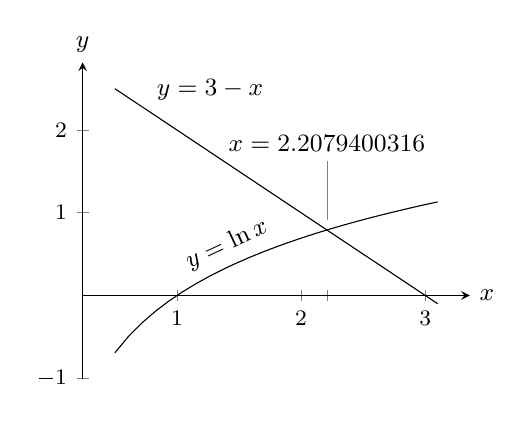
\begin{tikzpicture}[font=\small]
\begin{axis}[small,axis lines=middle,xlabel={$x$},ylabel={$y$},xlabel style={at={(current axis.right of origin)},anchor=west},ylabel style={at={(current axis.above origin)},anchor=south},enlargelimits=true,xtick={1,2,2.2079,3},xticklabels={1,2,,3}]
\addplot[domain=0.5:3.1]{ln(x)}node[pos=0.45,sloped,above]{$y=\ln x$};
\addplot[domain=0.5:3.1]{3-x}node[pos=0.1,above right]{$y=3-x$};
\draw(axis cs:2.2079,0.7921)node[pin={[pin distance=0.75cm]90:{$x=\num{2.2079400316}$}}]{};
\end{axis}
\end{tikzpicture}
\caption{نقطہ قطع}
\end{subfigure}\hfill
\begin{subfigure}{0.45\textwidth}
\centering
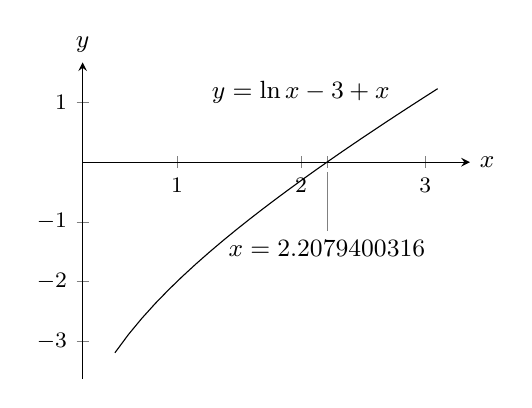
\begin{tikzpicture}[font=\small]
\begin{axis}[small,axis lines=middle,xlabel={$x$},ylabel={$y$},xlabel style={at={(current axis.right of origin)},anchor=west},ylabel style={at={(current axis.above origin)},anchor=south},enlargelimits=true,xtick={1,2,2.2079,3},xticklabels={1,2,,3}]
\addplot[domain=0.5:3.1]{ln(x)-3+x}node[pos=0.9,above left]{$y=\ln x-3+x$};
\draw(axis cs:2.2079,0)node[pin={[pin distance=0.75cm]-90:{$x=\num{2.2079400316}$}}]{};
\end{axis}
\end{tikzpicture}
\caption{جذر}
\end{subfigure}
\caption{تفاعل $f(x)$ اور $g(x)$ کے حل کی تلاش۔}
\label{شکل_تکمل_استعمال_نقطہ_قطع}
\end{figure}

\جزوحصہ{تبدیل ہوتے کلیات والا سرحد}
اگر سرحد کا کلیہ ایک یا ایک سے زیادہ نقطوں پر تبدیل ہوتا ہو تب ہم خطہ کو مطابقتی ذیلی خطوں میں تقسیم کرتے ہوئے ہر ذیلی خطے پر علیحدہ علیحدہ مساوات \حوالہ{مساوات_تکمل_استعمال_رقبہ_تعریف} کا اطلاق کرتے ہیں۔

\ابتدا{مثال}\شناخت{مثال_استعمال_تکمل_تبدیل_کلیہ}
ربع اول میں \عددی{y=\sqrt{x}} کے نیچے  اور \عددی{y=x-2} کے اوپر رقبہ تلاش کریں۔

حل:\quad
\موٹا{پہلا قدم:}\quad
ترسیم (شکل \حوالہ{شکل_مثال_استعمال_تکمل_تبدیل_کلیہ}) سے ہم دیکھتے ہیں کہ خطے کی بالائی سرحد \عددی{f(x)=\sqrt{x}} ہے جبکہ \عددی{0\le x\le 2}  پر اس کی نچلی سرحد \عددی{g(x)=0} اور \عددی{2\le x\le 4} پر نچلی سرحد \عددی{g(x)=x-2} ہے (نقطہ \عددی{x=2} پر \عددی{g(x)} کے دونوں کلیات ایک جیسے ہیں)۔ ہم \عددی{x=2} پر خطہ کو دو ذیلی حصوں \عددی{A} اور \عددی{B} میں تقسیم کر کے دونوں ذیلی خطوں کے لئے نمائندہ مستطیل بناتے ہیں۔\\
\موٹا{دوسرا قدم:}\quad
خطہ \عددی{A} میں تکمل کے حد \عددی{a=0} اور \عددی{b=2} ہیں۔ خطہ \عددی{B} کا بایاں حد \عددی{a=2} ہے۔اس کے دایاں حد جاننے کے لئے ہم مساوات  \عددی{y=\sqrt{x}} اور  \عددی{y=x-2} کو ایک ساتھ حل کرتے ہیں۔
\begin{align*}
\sqrt{x}&=x-2&&\text{\RL{$f(x)$ اور $g(x)$ کے برابر پر کریں}}\\
x&=(x-2)^2=x^2-4x+4&&\text{\RL{مربع لیں}}\\
x^2-5x+4&=0&&\text{\RL{ایک جانب منتقلی}}\\
(x-1)(x-4)&=0&&\text{\RL{تجزی}}\\
x=1,\quad x&=4&&\text{\RL{حل}}
\end{align*}
صرف \عددی{x=4} مساوات \عددی{\sqrt{x}=x-2} کو مطمئن کرتا ہے جبکہ مربع لینے کی وجہ سے حل \عددی{x=1} پیدا ہوا ہے جس کو رد کیا جاتا ہے۔ یوں دایاں حد \عددی{b=4} ہے۔\\
\موٹا{تیسرا قدم:}
\begin{align*}
f(x)-g(x)&=\sqrt{x}-0=\sqrt{x},&& 0\le x\le 2\\
f(x)-g(x)&=\sqrt{x}-(x-2)=\sqrt{x}-x+2,&&2\le x\le 4
\end{align*}
\موٹا{چوتھا قدم:}\quad
ہم خطہ \عددی{A} اور \عددی{B} کے رقبوں کا مجموعہ لیتے ہیں۔
\begin{align*}
S&=\int_0^2\sqrt{x}\dif x+\int_2^4(\sqrt{x}-x+2)\dif x\\
&=\big[\frac{2}{3}x^{3/2}\big]_0^2+\big[\frac{2}{3}x^{3/2}-\frac{x^2}{2}+2x\big]_2^4\\
&=\frac{2}{3}(2)^{3/2}-0+\big(\frac{2}{3}(4)^{3/2}-8+8\big)-\big(\frac{2}{3}(2)^{3/2}-2+4\big)\\
&=\frac{2}{3}(8)-2=\frac{10}{3}
\end{align*}
\انتہا{مثال}
%=========================
\begin{figure}
\centering
\begin{tikzpicture}[declare function={f(\x)=sqrt(\x);g(\x)=\x-2;}]
\begin{axis}[clip=false,axis on top,small,axis lines=middle,xlabel={$x$},ylabel={$y$},xtick={2,4},ytick={2,4},enlargelimits=true,xlabel style={at={(current axis.right of origin)},anchor=west},ylabel style={at={(current axis.above origin)},anchor=south}]
\addplot[name path=kfa,domain=0:0.5,draw=none]{f(x)};
\addplot[name path=kfb,domain=0.5:2,draw=none]{f(x)};
\draw[name path=axisfa](axis cs:0,0)--(axis cs:0.5,0);
\draw[name path=axisfb](axis cs:0.5,0)--(axis cs:2,0);
\addplot[fill=lgray] fill between [of =kfa and axisfa];
\addplot[fill=lgray] fill between [of =kfb and axisfb];
\addplot[domain=0:0.5]{f(x)};
\addplot[domain=0.5:4.2]{f(x)};
\addplot[domain=1.8:4.2]{g(x)}node[pos=0.75,right]{$y=x-2$};
\draw(axis cs:2.25,{f(2.25)})node[pin=135:{$y=\sqrt{x}$}]{};
\pgfmathsetmacro{\k}{1}
\pgfmathsetmacro{\w}{0.5}
\draw(axis cs:\k,{f(\k+\w/2)})--(\k+\w,{f(\k+\w/2)})coordinate(kTR)--(\k+\w,0)coordinate(kBR)--(\k,0)coordinate(kBL)--(\k,{f(\k+\w/2)})coordinate(kTL);
\draw[stealth-stealth]($(kBL)!0.75!(kTL)$)--($(kBR)!0.75!(kTR)$)node[pos=0.5,below]{$\Delta x$};
\draw(axis cs:\k+\w/2,{f(\k+\w/2)})node[circ]{}node[above]{$(x,f(x))$};
\draw(axis cs:\k+\w/2,0)node[circ]{}node[below,xshift=-0.75ex,yshift=-1ex]{$(x,g(x))$};
\draw(axis cs:2,{f(2)})--(axis cs:2,0);
\pgfmathsetmacro{\kk}{2.5}
\pgfmathsetmacro{\ww}{0.5}
\draw(axis cs:\kk,{f(\kk+\ww/2)})--(\kk+\ww,{f(\kk+\ww/2)})coordinate(kTR)--
(\kk+\ww, {g(\kk+\ww/2)})coordinate(kBR)--(\kk,{g(\kk+\ww/2)})coordinate(kBL)--(\kk,{f(\kk+\ww/2)})coordinate(kTL);
\draw[stealth-stealth]($(kBL)!0.75!(kTL)$)--($(kBR)!0.75!(kTR)$)node[pos=0.5,below]{$\Delta x$};
\draw(axis cs:\kk+\ww/2,{f(\kk+\ww/2)})node[circ]{}node[above,xshift=-0.5ex,yshift={0.5ex}]{$(x,f(x))$};
\draw(axis cs:\kk+\ww/2,{g(\kk+\ww/2)})node[circ]{}node[below right]{$(x,g(x))$};
\draw(axis cs:0.5,0.35)node[]{$A$};
\draw(axis cs:3.35,1.6)node[]{$B$};
\end{axis}
\end{tikzpicture}
\caption{خطہ برائے مثال \حوالہ{مثال_استعمال_تکمل_تبدیل_کلیہ}}
\label{شکل_مثال_استعمال_تکمل_تبدیل_کلیہ}
\end{figure}
\جزوحصہء{تکمل بلحاظ $y$}
